% Build the update pages from this directory:
%   xelatex -interaction=nonstopmode -halt-on-error CB_pricing_update_20260724.tex
% Run XeLaTeX twice, then prepend the resulting PDF to
% HISTORICAL_BASE_20260310.pdf to produce CB_pricing_full.pdf.
\documentclass[11pt,a4paper]{ctexart}

\usepackage[a4paper,margin=2.1cm,headheight=14pt]{geometry}
\usepackage{booktabs}
\usepackage{fancyhdr}
\usepackage{graphicx}
\usepackage{hyperref}
\usepackage{tabularx}
\usepackage[table]{xcolor}
\usepackage{enumitem}

\definecolor{navy}{HTML}{17365D}
\definecolor{blue}{HTML}{2F5597}
\definecolor{lightblue}{HTML}{D9EAF7}
\definecolor{lightgray}{HTML}{F2F4F7}
\definecolor{muted}{HTML}{5B6573}

\hypersetup{
  colorlinks=true,
  linkcolor=blue,
  urlcolor=blue,
  pdfauthor={Convertible Bond Pricing Research},
  pdftitle={中国可转债绝对定价研究：2026年7月更新}
}

\pagestyle{fancy}
\fancyhf{}
\lhead{\textcolor{muted}{中国可转债绝对定价研究}}
\rhead{\textcolor{muted}{数据截至 2026-07-24}}
\cfoot{\thepage}

\setlength{\parindent}{2em}
\setlength{\parskip}{0.35em}
\setlist[itemize]{leftmargin=2em,itemsep=0.25em}

\newcommand{\sectionbar}[1]{%
  \vspace{0.4em}
  {\color{navy}\Large\bfseries #1}\par
  \vspace{0.2em}
  {\color{blue}\rule{\textwidth}{1.2pt}}\par
}

\begin{document}

\begin{titlepage}
  \centering
  \vspace*{2.1cm}
  {\color{navy}\Huge\bfseries 中国可转债绝对定价研究\par}
  \vspace{0.45cm}
  {\color{blue}\LARGE Black--Scholes 与 Zheng--Lin 模型\par}
  \vspace{0.9cm}
  {\Large 研究结果更新版\par}
  \vspace{1.5cm}

  \renewcommand{\arraystretch}{1.45}
  \begin{tabular}{>{\bfseries}rl}
    数据截止日： & 2026-07-24 \\
    回测区间： & 2019-01-25 至 2026-07-24 \\
    调仓频率： & 月末调仓，共 90 个收益观察期 \\
    更新日期： & 2026-07-30 \\
  \end{tabular}

  \vfill
  \begin{minipage}{0.88\textwidth}
    \small\color{muted}
    本更新页以仓库内已生成并交叉核对的模型输出、策略结果和图表为依据。
    后附 2026-03-10 版本的完整研究正文，用于保留理论推导与历史研究框架；
    若历史正文中的回测数字与本更新页不一致，以本更新页为准。
  \end{minipage}
\end{titlepage}

\sectionbar{一、更新摘要}

本次更新将主报告的数据截止日由 2026 年 3 月推进至
\textbf{2026-07-24}，并使用当前仓库中的周频模型定价结果、月度因子回测
及同期一年期国债收益率口径重新核对绩效。研究仍聚焦两个已实现且可复现的
绝对定价模型：

\begin{itemize}
  \item \textbf{BS 模型：}闭式期权定价框架，主要反映正股价格、波动率、
        无风险利率与剩余期限对转债价值的影响。
  \item \textbf{ZL 模型：}基于蒙特卡罗路径并纳入已观测赎回、回售条款状态，
        同时使用信用利差对现金流折现。
\end{itemize}

\begin{table}[h]
  \centering
  \caption{最新回测结果：六因子等权多头组合（含双边 0.06\% 交易成本）}
  \rowcolors{2}{lightgray}{white}
  \begin{tabular}{lrrrrr}
    \toprule
    模型 & 年化收益 & 夏普比率 & 最大回撤 & 年化波动 & 平均换手率 \\
    \midrule
    BS & 19.41\% & 0.91 & -28.96\% & 19.21\% & 54.17\% \\
    ZL & 20.79\% & 0.95 & -29.75\% & 19.86\% & 57.15\% \\
    \bottomrule
  \end{tabular}
\end{table}

同期中证转债基准年化收益为 \textbf{7.14\%}。BS 与 ZL 六因子组合的
年化超额收益分别为 12.27\% 和 13.65\%。最新样本中 ZL 的收益和夏普略高，
但两类组合均经历接近 30\% 的最大回撤，因此模型定价信号不应被视为独立的
低风险套利。

\sectionbar{二、定价结果与最新截面}

截至 2026-07-24，BS 模型有 312 只有效定价，ZL 模型有 299 只有效定价。
在各自有效样本上，理论价格相对市场价格偏离度的截面中位数分别为
\textbf{-8.20\%} 与 \textbf{-19.16\%}。该结果说明当前绝对定价模型普遍给出
低于市场价格的估值，但不能直接解释为可无摩擦做空的套利空间：流动性、
信用风险、条款执行意愿、波动率估计误差和卖空约束都会影响偏离的可交易性。

\begin{figure}[p]
  \centering
  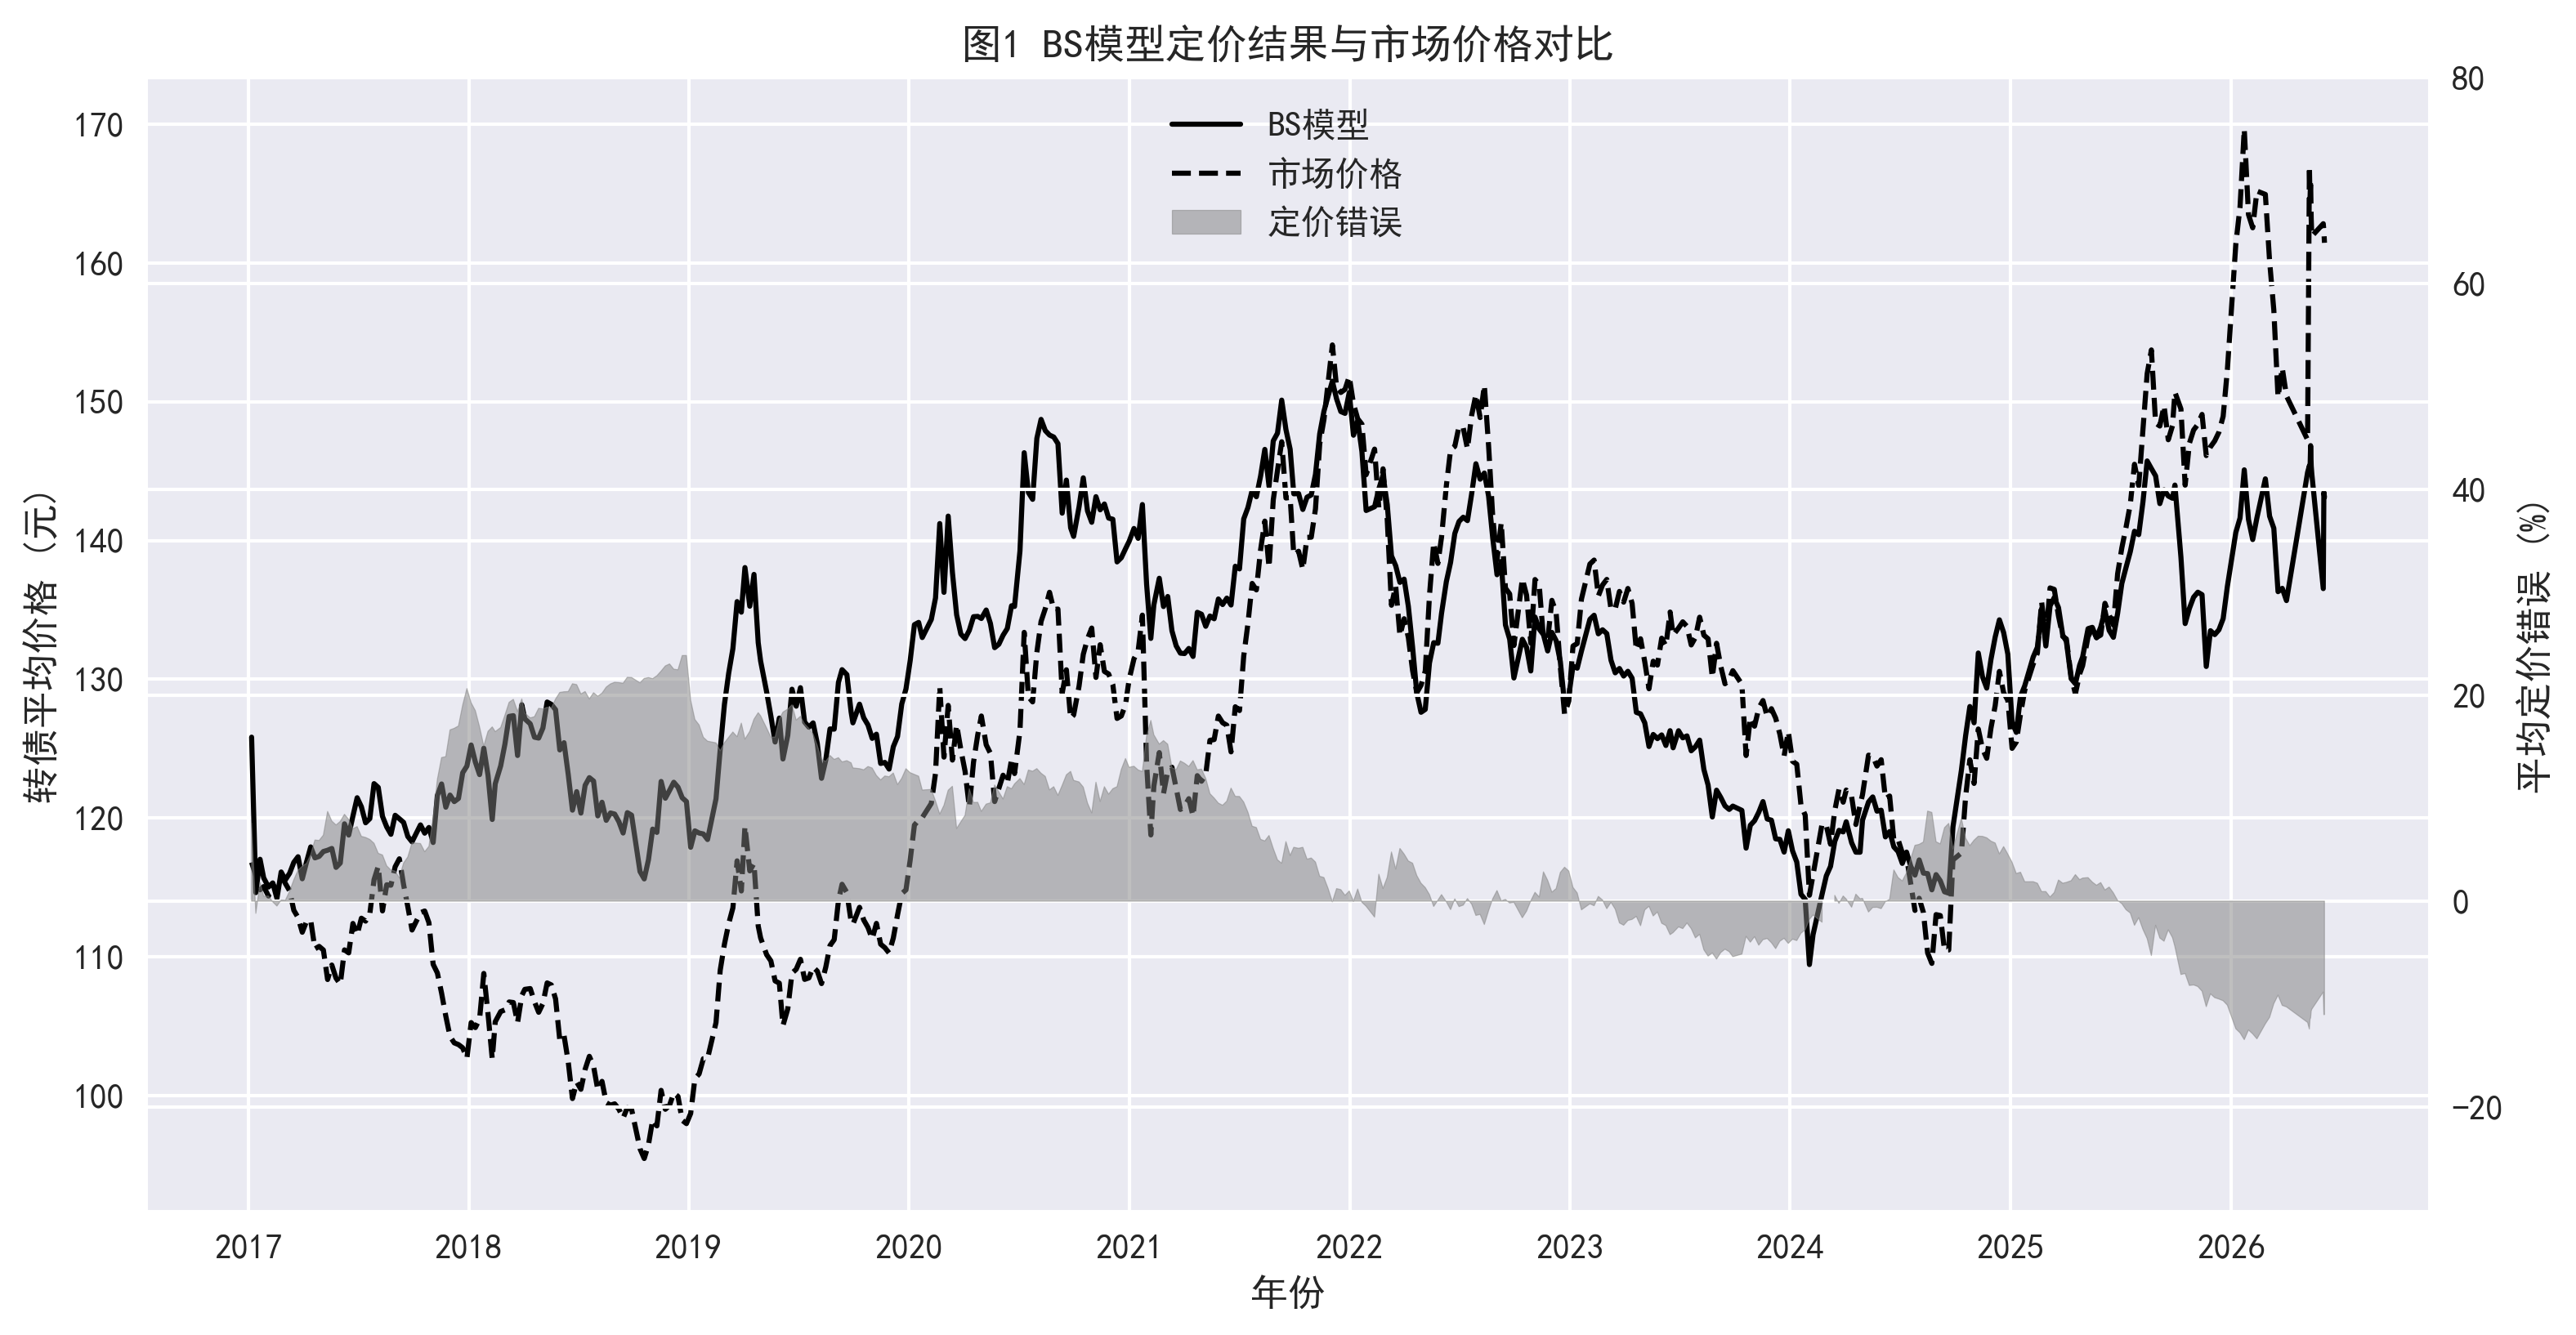
\includegraphics[width=0.94\textwidth]{../backtest/Fig1_BS_Price_Time_Series.png}
  \caption{BS 模型理论价格、市场价格与相对偏离度}
  \vspace{0.8cm}
  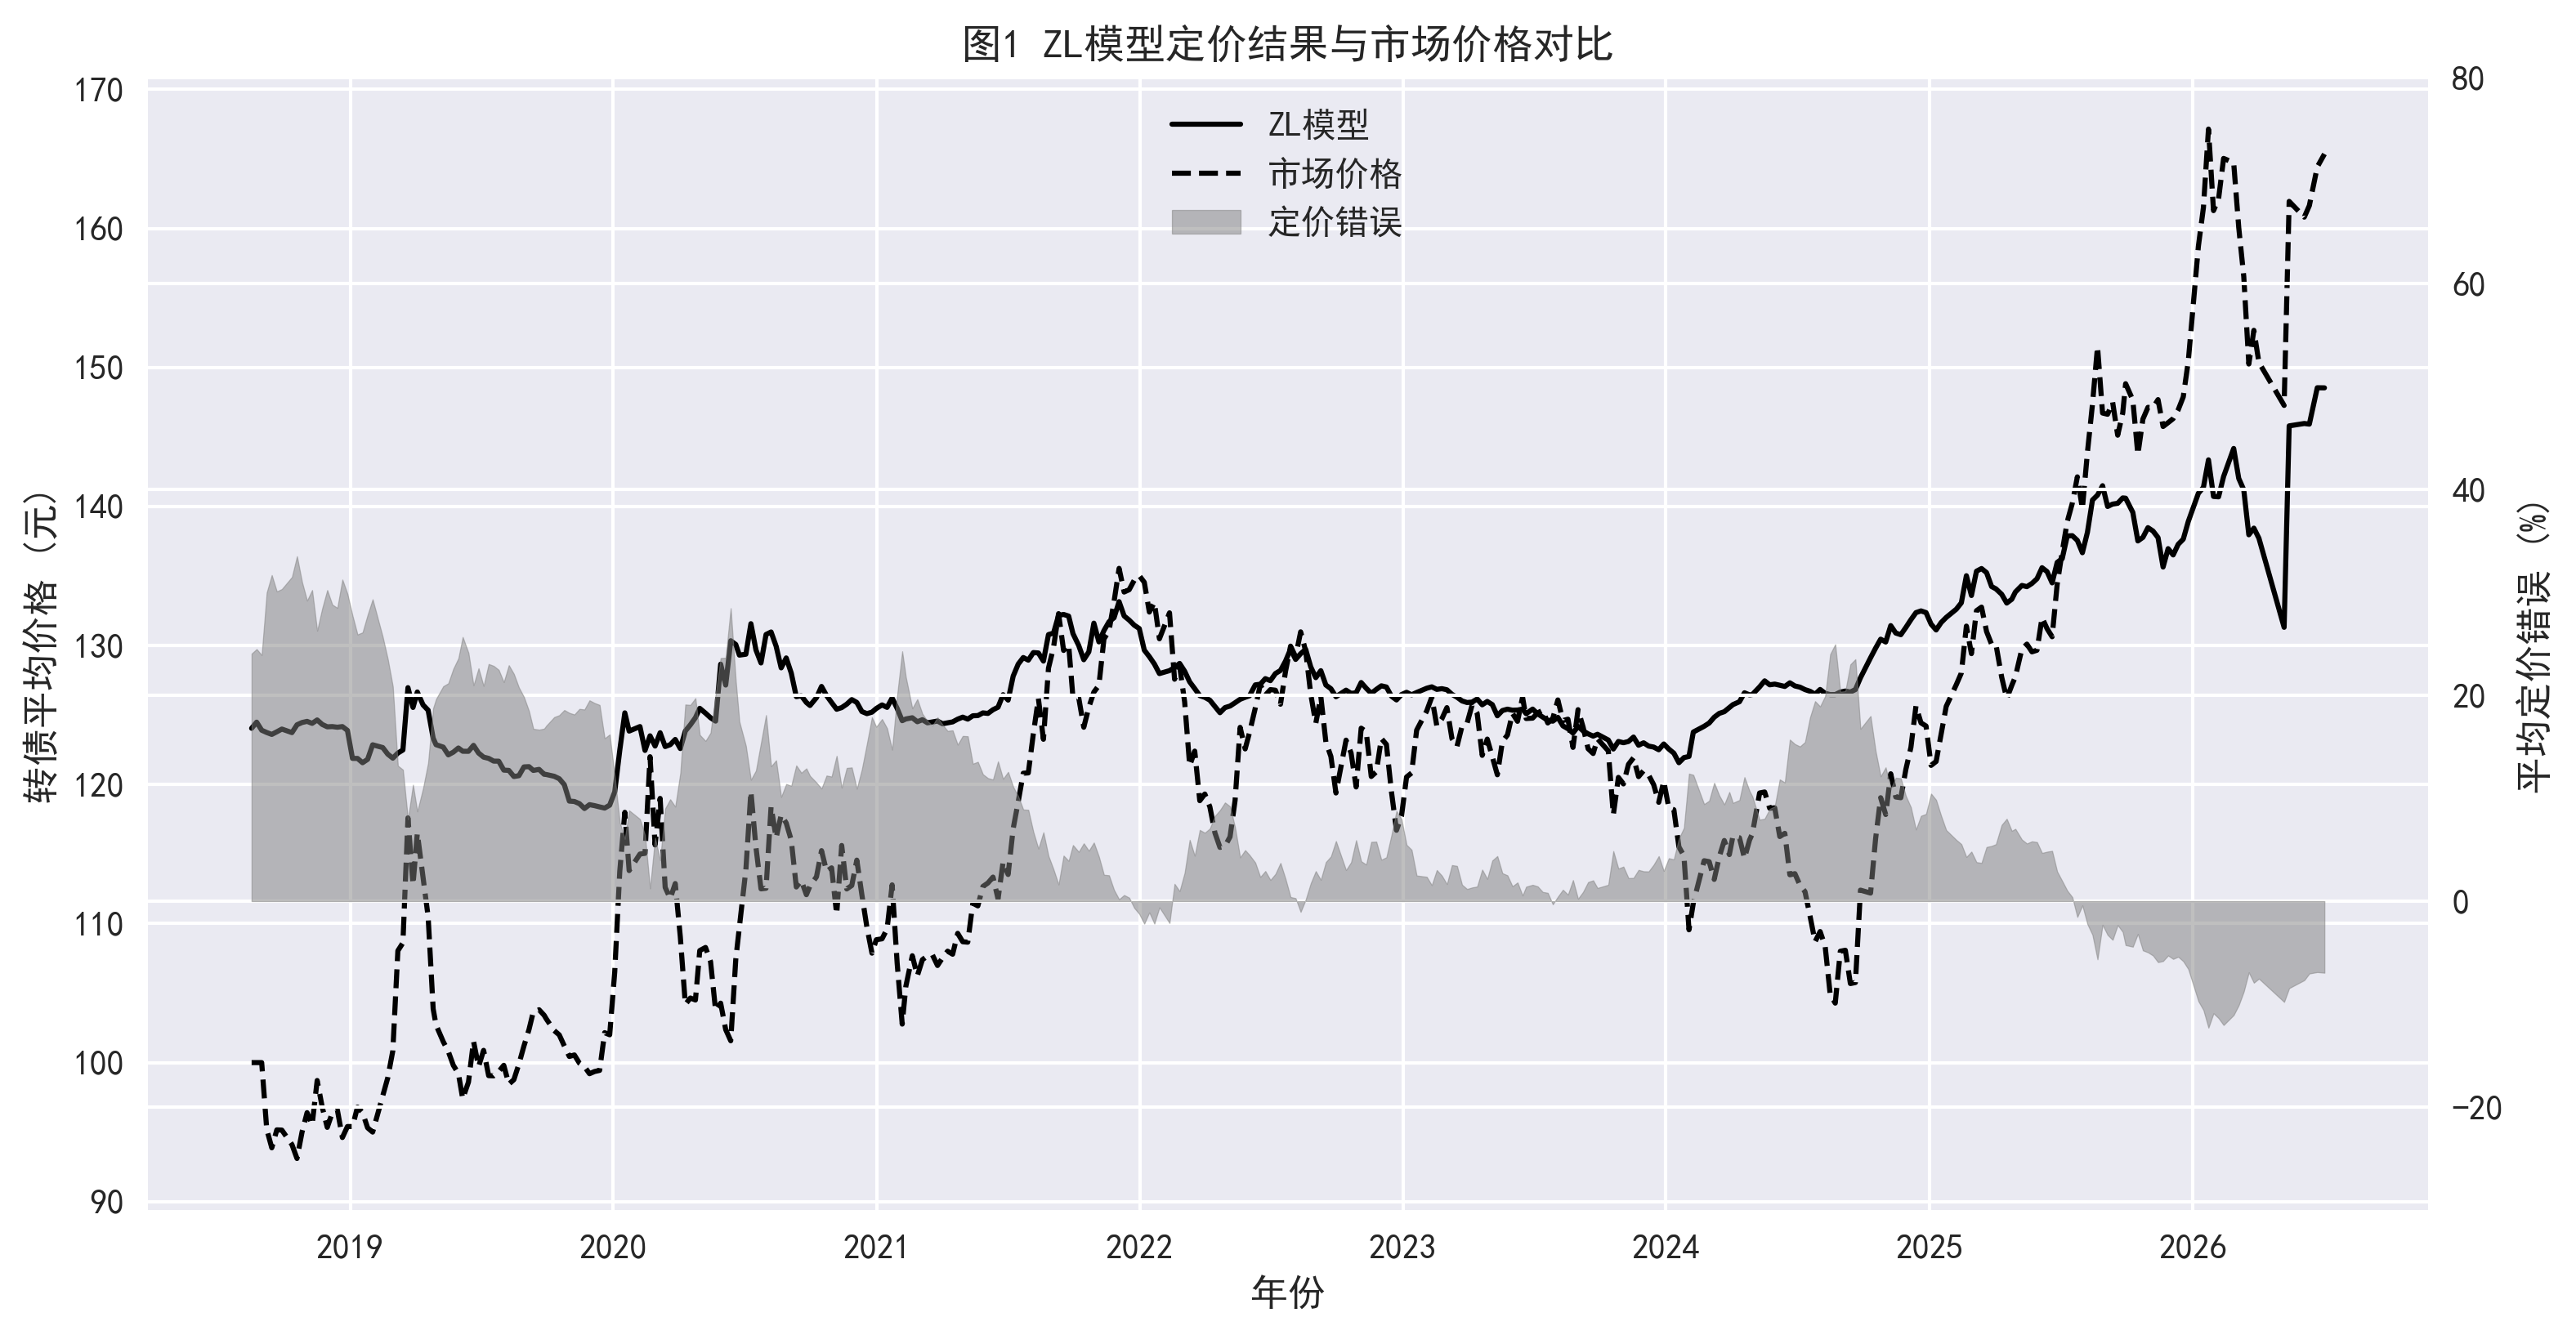
\includegraphics[width=0.94\textwidth]{../backtest/Fig1_ZL_Price_Time_Series.png}
  \caption{ZL 模型理论价格、市场价格与相对偏离度}
\end{figure}

\clearpage
\sectionbar{三、策略表现}

策略每月按六个标准化因子等权合成后选取多头组合。六个因子包括流动性、
波动率、量价相关性、估值、动量和相应模型的定价偏差。收益结果使用月度
持有期收益，并扣除双边 0.06\% 交易成本。

\begin{table}[h]
  \centering
  \caption{定价偏差单因子与六因子合成结果}
  \rowcolors{2}{lightgray}{white}
  \begin{tabular}{llrrrr}
    \toprule
    模型 & 策略 & 年化收益 & 夏普比率 & 最大回撤 & 累计收益 \\
    \midrule
    BS & 定价偏差单因子 & 20.52\% & 1.20 & -21.76\% & 304.91\% \\
    BS & 六因子等权 & 19.41\% & 0.91 & -28.96\% & 277.87\% \\
    ZL & 定价偏差单因子 & 22.92\% & 1.41 & -14.99\% & 369.45\% \\
    ZL & 六因子等权 & 20.79\% & 0.95 & -29.75\% & 311.85\% \\
    \bottomrule
  \end{tabular}
\end{table}

定价偏差单因子在当前样本中的风险调整后表现优于六因子等权组合，尤其是
ZL 定价偏差因子。不过，这些结果来自同一历史样本内的描述性回测，尚不构成
样本外稳健性或未来收益保证。

\begin{figure}[p]
  \centering
  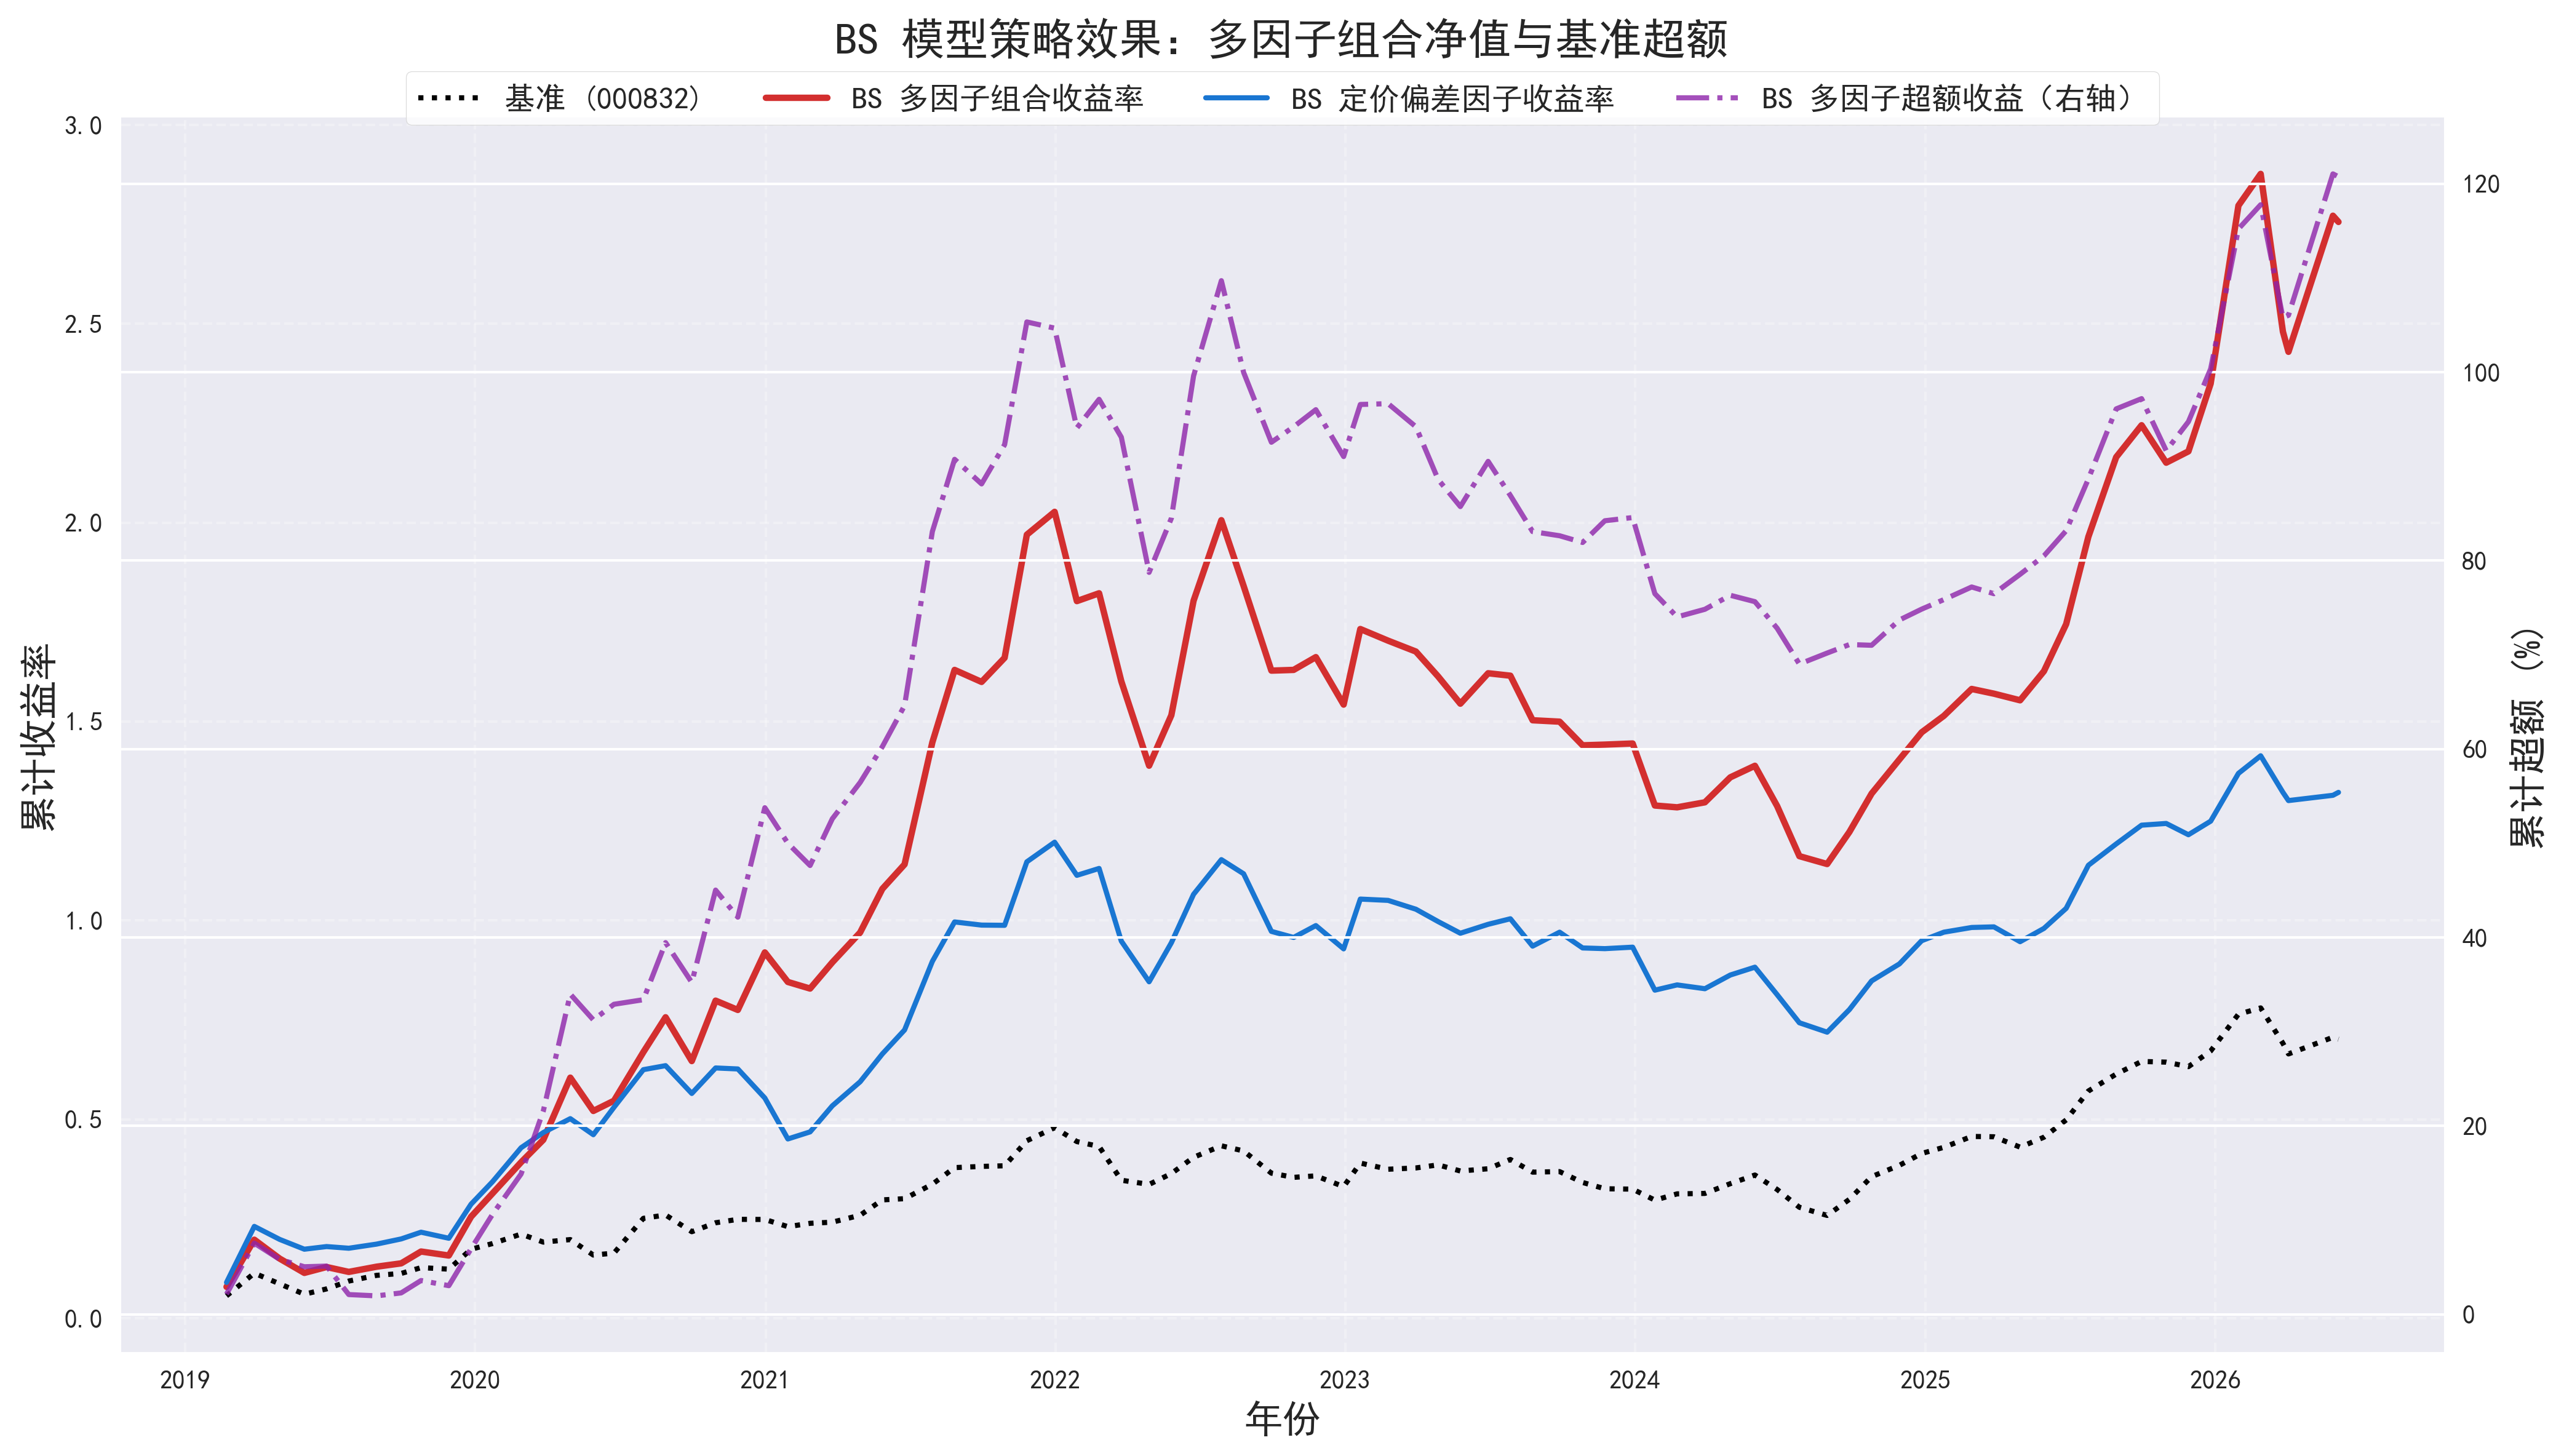
\includegraphics[width=0.95\textwidth]{../long-short strategy/BS_model_performance.png}
  \caption{BS 定价偏差策略与基准净值}
  \vspace{0.8cm}
  \includegraphics[width=0.95\textwidth]{../long-short strategy/ZL_model_performance.png}
  \caption{ZL 定价偏差策略与基准净值}
\end{figure}

\clearpage
\sectionbar{四、因子关系与解释边界}

错误定价因子与流动性、波动率、量价、传统估值及动量因子共同进入组合。
相关性图用于判断定价偏差是否仅仅复制已有风格暴露。相关性较低只能说明
线性重合有限，不能替代因果识别、样本外检验或容量分析。

\begin{figure}[h!]
  \centering
  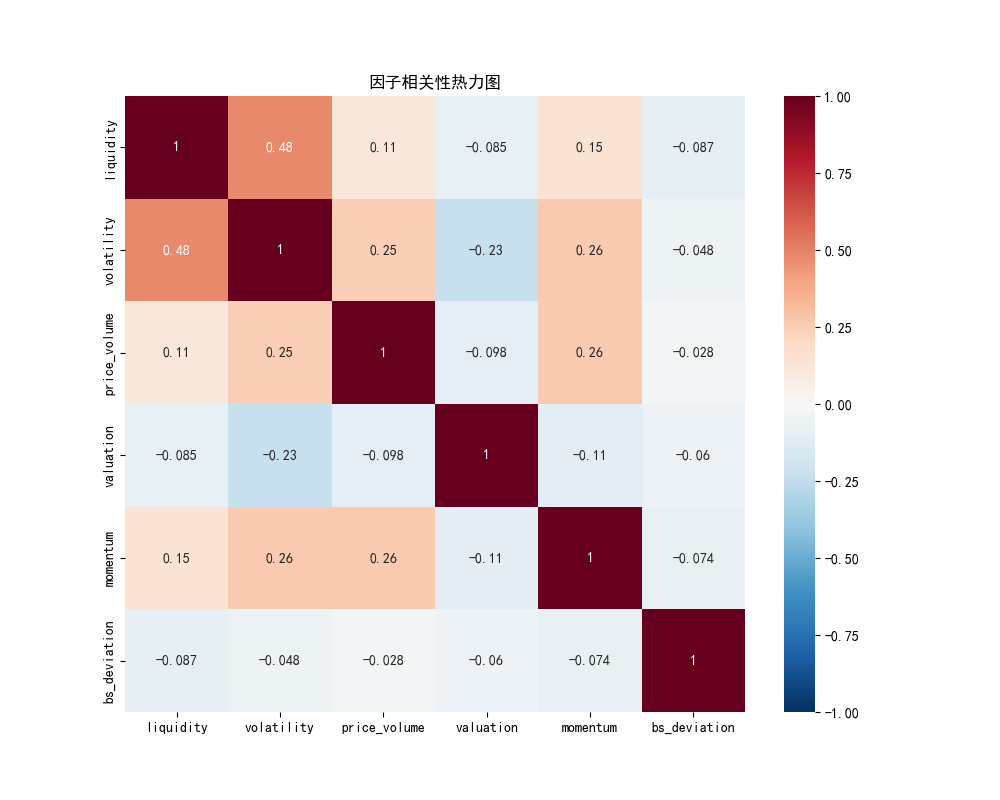
\includegraphics[width=0.64\textwidth]{../mispricing factor/BS_factor_correlation.png}
  \caption{BS 定价偏差与五类传统因子的相关性}
  \vspace{0.15cm}
  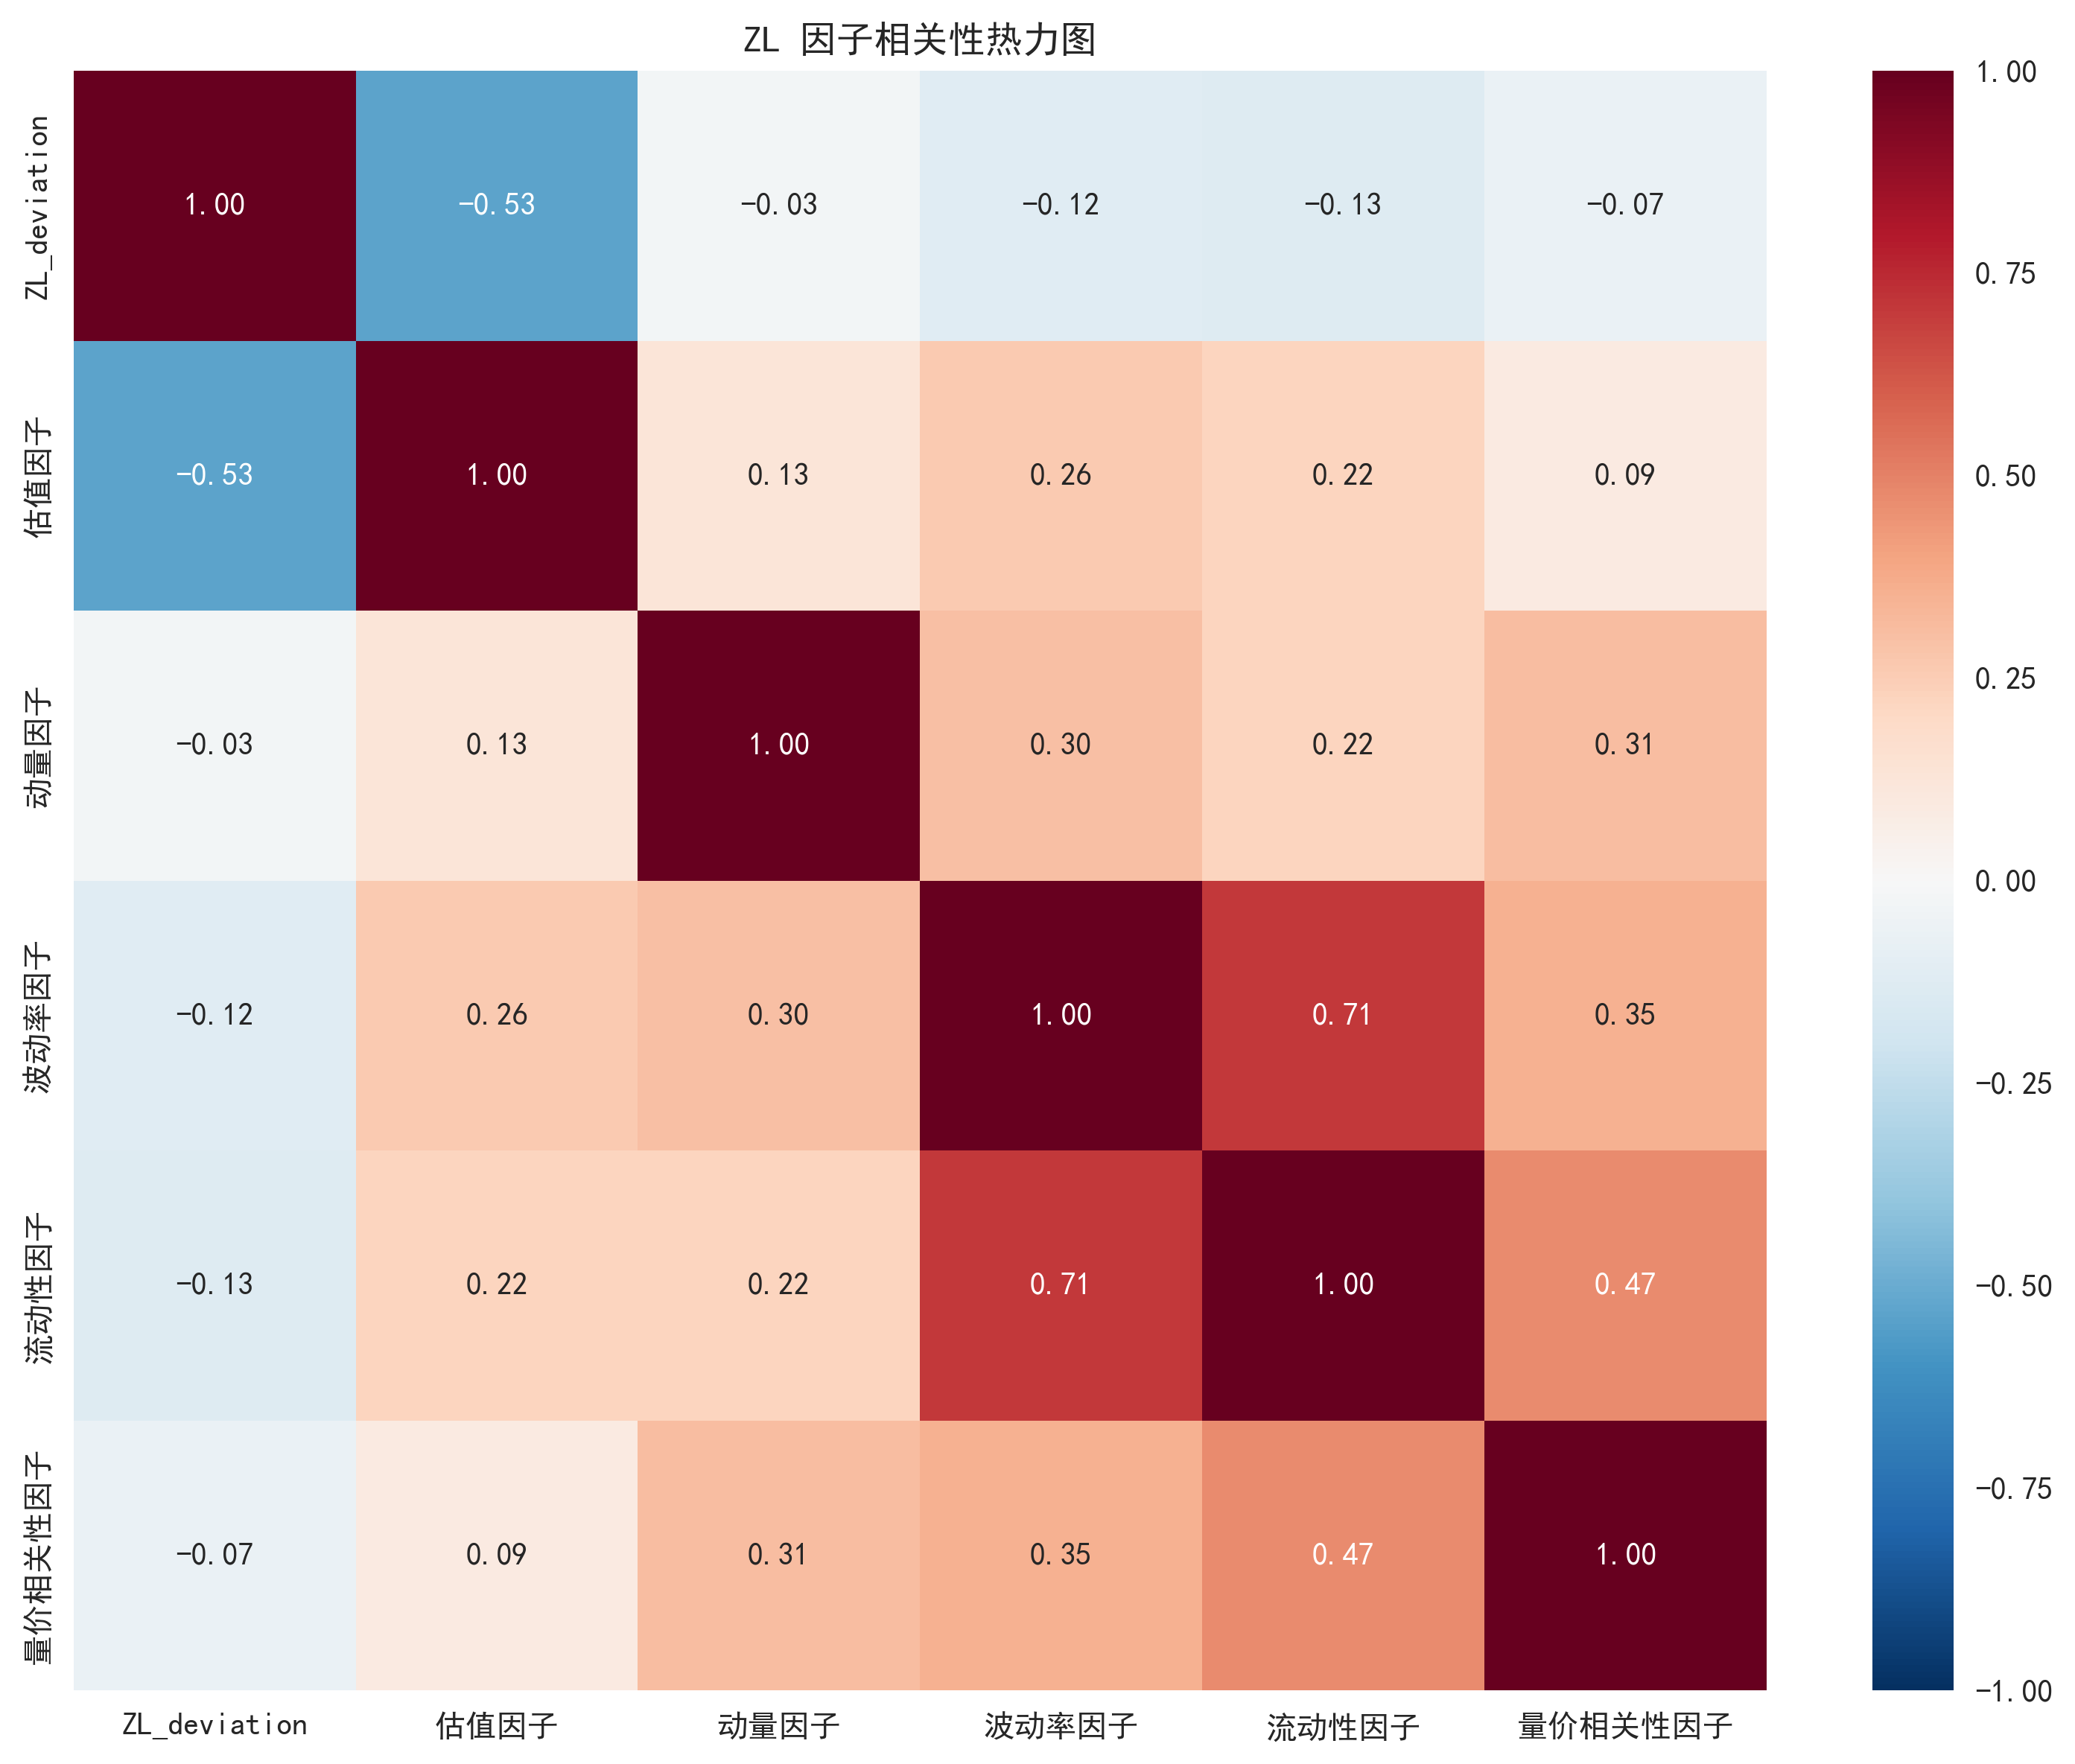
\includegraphics[width=0.64\textwidth]{../mispricing factor/ZL_factor_correlation.png}
  \caption{ZL 定价偏差与五类传统因子的相关性}
\end{figure}

\clearpage
\sectionbar{五、数据与复现口径}

\begin{tabularx}{\textwidth}{>{\bfseries}p{3.2cm}X}
  \toprule
  项目 & 当前口径 \\
  \midrule
  市场数据 & Tushare 可转债日行情、基础信息、评级、财务指标及正股数据；
             AkShare 国债收益率曲线。 \\
  模型观察频率 & 每个已完成交易周保留一个实际交易日定价截面。 \\
  策略调仓 & 月末调仓，收益期从 2019-01-25 开始，最后一个观察期结束于
             2026-07-24。 \\
  交易成本 & 多头因子回测扣除双边 0.06\% 交易成本。 \\
  夏普口径 & 使用回测期内实际观测的一年期国债收益率均值作为无风险利率。 \\
  输出依据 & \texttt{BS/ZL\_Model\_Summary.xlsx}、
             \texttt{B-S/Z-L\_alpha\_strategy\_results.csv} 与对应绩效表。 \\
  \bottomrule
\end{tabularx}

\sectionbar{六、LSM 模型状态说明}

东北证券《可转债研究框架：从理论概念到实战策略》还介绍了第三种绝对定价
方法 LSM（最小二乘蒙特卡罗）。LSM 通过回归估计继续持有价值，并与即时转股
价值比较，以处理美式提前转股权。

\textbf{本仓库当前没有 LSM 实现或 LSM 回测输出，因此本报告不展示 LSM
绩效，也不把其列为已完成模型。} 若后续加入 LSM，需要先固定回归基函数、
路径数量、提前转股规则及赎回、回售、下修事件顺序，再按与 BS/ZL 相同的数据
截止日和交易成本口径进行比较。

\sectionbar{七、风险提示与结论}

\begin{itemize}
  \item 模型价格依赖波动率、信用利差和条款行为假设，参数误差可能形成长期、
        不可收敛的定价偏离。
  \item 中国可转债卖空和对冲机制有限，理论高估不等于可实现的空头收益。
  \item 回测存在样本内选择、存续样本结构变化、流动性和容量约束。
  \item 当前结果支持将 BS 与 ZL 作为互补定价锚，但仍需风险预算、市场状态
        约束和样本外检验。
\end{itemize}

\vfill
\begin{center}
  \color{muted}
  \rule{0.75\textwidth}{0.5pt}\\[0.6em]
  \large 历史完整研究正文自下一页开始\\
  \small 历史正文报告日期为 2026-03-10；最新结果以此前更新页为准。
\end{center}

\end{document}
